\chapter{Integration Into Machine Translation Systems}
\label{chap:integration}
In this chapter, we demonstrate how our CL-WSD techniques can be integrated
into running machine translation systems, with the goal of improving lexical
selection in practice, while minimizing code changes to the MT software. We
translate from Spanish to Guarani with Moses\cite{koehn-EtAl:2007:PosterDemo},
an off-the-shelf phrase-based statistical MT system, and from Spanish to
Quechua with SQUOIA\cite{rios2015basic}, a primarily rule-based MT system
developed by Rios \emph{et al.} at the University of Zürich. These two
integrations are meant to be simple proofs of concept, rather than an attempt
to define a best practice, but they demonstrate at least conceptually how
CL-WSD can be used with these kinds of translation systems. Afterwards, we look
at evaluating Chipa's effect on MT output in both of these use cases.

A common thread in the MT settings addressed in this work is that there is a
relatively small amount of text available for training a target-side language
model, so we should not rely on the LM on its own for making
contextually-appropriate word choices. This problem is especially significant
for RBMT systems without weights built into their lexicons; many translation
options will be licensed for a given input word, and selecting among them can
be difficult. In SQUOIA, for example, there are some rules for lexical
selection, but they were written by hand and only cover a small subset of the
vocabulary and a limited number of contexts.

The difficulty of resolving these ambiguities is mitigated for statistical
machine translation systems for language pairs with large bilingual corpora, as
large n-gram language models and phrase tables containing common multi-word
expressions can encourage coherent word choices. However, for most language
pairs these resources are not available; as a result, many research groups,
have sought to build MT systems with rule-based approaches for under-resourced
language pairs.

In cases where some training data is available, though, we can investigate
combining machine learning and rule-based approaches, resulting in hybrid MT
systems that can benefit from the small, but potentially growing resources for
the relevant language pair. These could include bitext corpora for the language
pair, or with techniques like the ones described in Chapters
\ref{chap:monolingual} and \ref{chap:multilingual}, monolingual source-language
corpora and tools, or even bitext matching the source language with other
target languages. So adding trained CL-WSD classifiers to existing lexical
selection rules can allow our MT systems to find regularities that may not be
obvious to human rule-writers, providing lexical selection guidance for word
types with sufficient coverage in the training corpus.

With these additional classifiers, a primarily RBMT system can take advantage
of statistical evidence without significantly changing its design, and to
improve its word choices as additional bitext or other resources become
available.
WSD techniques can also be applied to statistical machine translation, as has
been shown by, for example, Carpuat \emph{et al.} \cite{carpuatpsd} and Tamchyna
\emph{et al.} \cite{tamchyna2014integrating}. In this chapter we demonstrate
specifically how to add the Chipa CL-WSD system to Moses, for a language pair
with an under-resourced target language.

Among other pieces of software related to this work, especially the corpus
preparation scripts, the code to integrate Chipa into these machine
translation systems is in a package called Tereré \footnote{Available at
\url{http://github.com/alexrudnick/terere} ; Tereré is a cold variety of yerba
mate brewed with ice water; it is a specifically Paraguayan specialty.}.


\section{Integrating Chipa into Phrase-Based Statistical Machine Translation}
Moses\footnote{Available at \url{http://statmt.org/moses/}} is a mature,
well-maintained and popular statistical machine translation package, in broad
use for both research and practical purposes.
Like many SMT systems, Moses combines signals from different subcomponents when
searching through the space of possible translations for an input sentence. It
does this using a log-linear model, in which each component scores a candidate
translation, and then the scores from the different components are combined in
a weighted sum. Some typical components are the probabilities learned for a
given phrase during phrase extraction (without regard to context) in both
translation directions, scores from the target-language language model, learned
distortion models that reflect estimated differences in word order between
source and target languages, and a handful of other features\footnote{For an
overview of techniques commonly used in phrase-based statistical MT, please see
Koehn's book on the subject \cite{koehn2010statistical}.}.

Conveniently for our work here, Moses includes an interface for adding new
feature functions\footnote{See
\url{http://www.statmt.org/moses/?n=Moses.FeatureFunctions} for documentation.}
to be combined in the log-linear model, so we can add new information to help
guide the decoding process.

Scores in this framework are expected to represent log probabilities, meaning
that, concretely, they are real numbers less than 0, as the logarithm of a
number between 0 and 1 will be negative. The decoder's beam search procedure
then attempts to maximize the total score for a translation, which means
finding a translation with a score as high as possible, \emph{i.e.}, maximally
close to 0.

We built a simple phrase-based SMT system with Moses and used this feature
function API to have Chipa evaluate candidate translations. For simplicity, we
added a constraint in the Moses phrase-extraction system so that the source
side of all phrases must be at most one token long, to match the alignments
used in the previous chapters.

During the search through the space of possible translations, Moses proposes
candidate translations for each source word to the Chipa feature function, and
this function returns a score based on how likely the translation seems to the
CL-WSD system, considering the source-language sentence context. This score is
returned to Moses, which combines all of the available features in a log-linear
combination.

The weights for all of the features provided to the system (translation
probabilities, LM scores, CL-WSD scores, and perhaps others) are typically
tuned on a development set with Minimum Error-Rate Training, or ``MERT"
\cite{och:2003:ACL} ; thus, if CL-WSD scores turn out to be useful for
achieving high BLEU scores on the development set sentences, Chipa's feature
function will be assigned a higher weight. If not, its advice carries less
weight, than, for example, that of the language model.

\subsection{Interfacing between Moses and Chipa}
The Moses decoder is written in C++, and the typical approach for adding new
feature functions is to write new C++ classes, which are linked in with the
decoder binary. However, the Chipa software is built in Python, so for
simplicity, we implemented a protocol for communication between the Moses C++
code and the Chipa server, based on Unix pipes\footnote{In earlier work with
SQUOIA \cite{rudnick:saltmil2014}, we had communicated between Chipa and a
machine translation system with XML-RPC
\footnote{\url{http://xmlrpc.scripting.com/}}, but for simplicity of
implementation, here we built a new text-based protocol.}; see Figure
\ref{fig:moses-chipa-diagram} for a visual aid.  Named Unix pipes, or FIFOs,
allow the creation of a special kind of filesystem object whereby messages can
be passed between processes in the same computer. Here Moses requests an
evaluation for a certain translation of a source-language phrase given the
source-language sentence as context, and Chipa returns a score based on how
likely it considers that phrase, represented as log probabilities.

Moses also allows for phrase tables to contain arbitrary annotations in its
phrase table, and one might ask whether it would be possible to avoid the
trouble of implementing a new feature function in C++, when we could simply
add features to a translation of a phrase, in the phrase table on disk.
However, this misses the point of using our CL-WSD classifiers -- we want to
know about which translation is most appropriate for a given source-language
phrase, \emph{in this context}. We could imagine running our classifiers as a
preprocessing step, and simply producing a phrase table specific to each
individual sentence that we want to translate, but there could be multiple
instances of a source phrase in a single input sentence. So here we run our
classifiers during decoding, using the current source sentence as context.

\begin{figure}
  \begin{centering}
  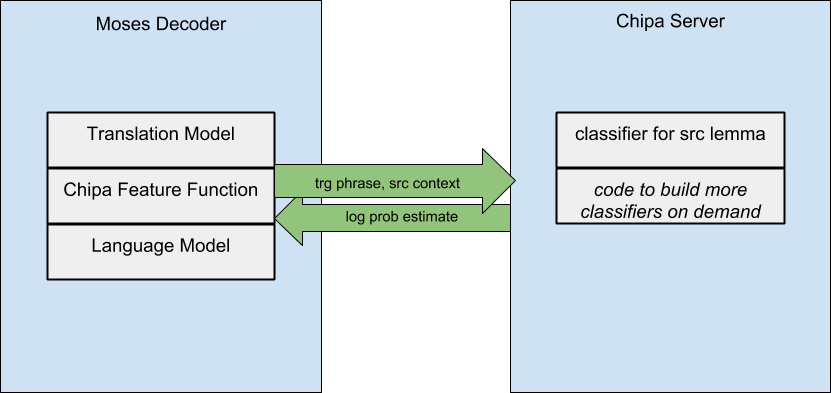
\includegraphics[width=15cm]{moses-chipa-diagram.png}
  \end{centering}
  \caption{Schematic diagram showing the relationship between the Moses decoder
  process, running the custom-made Chipa feature function, which communicates
  with the Chipa server process. The Chipa server returns probability
  estimates for proposed target-language phrases based on the given
  source-sentence context, when available.}
  \label{fig:moses-chipa-diagram}
\end{figure}

\section{Integrating Chipa into Rule-Based Machine Translation}

\subsection{The SQUOIA RBMT system}
SQUOIA\footnote{Code available at \url{https://github.com/a-rios/squoia} ;
the project is more broadly described at
\url{https://www.cl.uzh.ch/en/research/machine-translation/hybridmt.html}}
is a system for machine translation, primarily from Spanish to the Cuzco
dialect of Quechua, which is spoken around the Peruvian city of Cuzco.

SQUOIA was developed by a team at the University of Zurich. For the most part,
it is a classical rule-based system, although the team has added machine
learning techniques to a few subcomponents, such as predicting verb morphology
for cases when its rules cannot reliably disambiguate
\cite{riosgonzales-gohring:2013:HyTra}. It does not, by default, use machine
learning for lexical selection as such, although it does include a language
model to help select among the translations licensed by its transfer rules.
Also its initial input analysis stages call open-source NLP tools based on
learned models. SQUOIA uses FreeLing \cite{padro12} for morphological analysis
and named-entity recognition, Wapiti \cite{lavergne2010practical} for tagging,
and DeSr \cite{attardi-EtAl:2007:EMNLP-CoNLL2007} for parsing.

SQUOIA's architecture is based on the Matxin system \cite{matxin2005}, which
was originally intended for translating from Spanish to Basque. It consists of
a pipeline of smaller steps, each of which passes along a tree describing the
current input text and transformations that have been applied to it, in XML
form. As the steps progress, the input Spanish is analyzed and gradually
transformed into Quechua output. Many modules focus on very particular aspects
of the representation, leaving most of their input unchanged; for example, one
phase performs coreference resolution, and another phase uses rules to try to
decide whether an instance of the Spanish preposition \emph{de} should be
translated into Quechua as indicating the ablative case (direction of motion),
or the genitive case (posession). Please see Figure \ref{fig:squoia-steps} for
an overview of the most important steps in the SQUOIA pipeline.

%% XXX working here
In order to integrate Chipa CL-WSD into SQUOIA, we added an additional
intermediate step to the pipeline that reads the XML representation of the
current state of the transformation, occurring just after rule-based lexical
disambiguation. This new module extracts the original Spanish input text from
the intermediate representation and finds lexical-selection ambiguities that we
can attempt to resolve with Chipa, \emph{i.e.}, nodes in the tree where there
are several possible Quechua lemmas that could be chosen as a translation. It
then calls the Chipa CL-WSD classifiers to get an estimated probability
distribution over possible translations for that input focus word, in its
particular context.

For each such node with such multiple translation possibilities, we look at
each of the translations under consideration by SQUOIA, and if any of them was
the top classification output from the Chipa classifiers, we constrain SQUOIA
to take that choice by removing the other available options.
We then update the XML tree to pass the choices along to subsequent steps.

If there are no such overlapping translations, or if no Chipa classifier was
available for that word, we make no changes to the input tree, and allow SQUOIA
to proceed as normal. Notably, since Chipa and SQUOIA do not share the same
lexicon and bitext alignments may be noisy, translations observed in the bitext
may be unknown to the SQUOIA system, and lexical entries in the SQUOIA
dictionary may not be attested in the training data.

\begin{figure}
  \begin{itemize}
  \item Tokenization, morphological analysis, tagging, parsing.
  \item Disambiguating Spanish verbs with rules that match on contextual clues
  (low recall; the rules are manually crafted by linguists)
  \item Disambiguating Spanish verbs with an SVM classifier.
  \item Lexical lookup and transfer: insert all possible translations for every
  input token from the bilingual dictionary.
  \item Rule-based disambiguation, attempting to eliminate possible
  lexical-selection ambiguities and morphological choices. (similarly low
  coverage; it is not feasible for linguists to write rules for all possible
  contexts for every word type in the lexicon)
  \item \emph{DISAMBIGUATION WITH CHIPA INSERTED HERE}
  \item Syntactic transfer, building more Quechua-like syntactic structures
  (rule-based).
  \item Reordering based on new syntactic trees (rule-based).
  \item Use KenLM language models trained over Quechua words and morphemes to
  choose most likely alternatives remaining.
  \item Morphological generation: produce Quechua surface forms with a finite
  state transducer, output n-best list.
  \end{itemize}

  \caption{An overview of the steps in the SQUOIA MT system; there are a few
  more, handling specific circumstances and parts of speech.}
  \label{fig:squoia-steps}
\end{figure}


\section{Translation Evaluation for Spanish-Guarani}

%% TODO: explain how we sampled test sets, what it means that we picked verses
%% rather than sentences

\subsection{Results: BLEU scores for Spanish-Guarani}

In Figure \ref{fig:bleu-es-gn}, we report BLEU scores for our PBMT system with
Chipa enabled.
%% TODO Explain what's up with training with MERT and then turning off that
%% feature.

\begin{figure*}
  \begin{centering}
  \begin{tabulary}{\textwidth}{|R|L|}
    \hline
    setting & BLEU \\
    \hline
    Moses with Chipa enabled &  16.24 \\
    \hline
    Same system, with Chipa disabled &  10.01 \\
    \hline
  \end{tabulary}
  \end{centering}
  \caption{BLEU scores on our Spanish-Guarani test set. Note that this is
  translating to \emph{lemmatized} Guarani, rather than having to predict
  fully-inflected forms.}
  \label{fig:bleu-es-gn}
\end{figure*}


\section{Translation Evaluation for Spanish-Quechua}

In order to evaluate the effect of Chipa on lexical selection in a live
translation task, we used SQUOIA to translate a hundred verses sampled from our
Spanish-Quechua Bible bitext, both in its default settings, and with the
addition of Chipa. The addition of SQUOIA resulted in some change for the
SQUOIA output for 55 of the 100 verses translated; some of the changes were
only in order or punctuation, but the majority were local differences in word
choice.

The BLEU scores for SQUOIA output on this test set were quite low (lower than
one BLEU point), and were not improved by adding Chipa's CL-WSD. But this is a
rather more difficult task, since we are attempting to generate fully-inflected
Quechua surface forms, rather than selecting appropriate lemmas, and BLEU
scoring requires us to match n-grams exactly, which is made less likely by the
rich morphology, including evidential markers, of Quechua. Additionally, as
Rios notes \cite[\S 5.9]{rios2015basic}, translations into Quechua tend to be
fairly free, rather than close analogues of the source Spanish.

In any case, here we will show examples of word choices that were changed with
the addition of Chipa CL-WSD, and, armed with our Spanish-Quechua dictionary
\cite{academiamayor}, determine whether they are more or less appropriate than
the choices that the SQUOIA system would have made on its own. For some
examples chosen from the sampled test set, see Figure
\ref{fig:some-spanish-verses-with-changes}.

%% TODO: put counts of how many verses changed, and how many of the changes
%% were clearly good, clearly bad, and unclear from my perspective.

One pattern that we find among the changed output is that Chipa tends to
encourage SQUOIA to choose \emph{churi} (a son, when discussed with regard to
his father) rather than the more generic \emph{wawa}, which can refer to any
child; for most of the test sentences where we saw this change happen, it
seemed like an appropriate choice. For example, in Sentence
\ref{sent:putyourhand}, we are referring to a son of a particular man, so this
seems like a good choice.

We see when translating Sentence \ref{sent:alreadydead}  from Spanish to
Quechua, without Chipa, SQUOIA translates \emph{llamando} ('calling') to
\emph{sutikuspa}, where \emph{suti} is the sense of ``llamar" that refers to
naming. However, with Chipa, SQUOIA picks \emph{waqyaspa}, where \emph{waqyay}
is the communicative sense, rather than the naming sense.

Many changes caused by Chipa seem to be different choices among near synonyms.
For example, in Sentence \ref{sent:burning}, without Chipa, we translate
\emph{ardiente} as \emph{k'anaq}, which seems to be a good translation, meaning
``glowing, ardently burning". With Chipa, it becomes \emph{'yawraq'} 'burning,
glowing'. And one difference revealed an ambiguity in Spanish that is clearly
distinguished in Quechua: in Sentence \ref{sent:reins}, without Chipa, we
translate \emph{labios} 'lips' as an inflection of \emph{wirp'a}, which
apparently only refers to the lower lip; with Chipa, we choose an inflection of
\emph{sirphi}, which seems to refer to only the upper lip
\footnote{Also, more modern English translations seem to choose something like
``innermost being" rather than referring to one's innards, but the King James
Version uses the term ``reins", which apparently historically referred to the
kidneys.}.

We note in Sentence \ref{sent:llama} a serious word-sense issue that Chipa did
not manage to fix; in both cases, SQUOIA failed to interpret \emph{llama} as
'flame'\footnote{The Spanish token \emph{llama} can be an inflection of the
verb \emph{llamar} 'to call', or as a noun, 'flame', or of course it can refer
to llama the animal, which is a loan word from Quechua.}; this seems to be a
cascading error from part-of-speech tagging, as SQUOIA's bundled tagger marked
it as a verb. In any case, without SQUOIA, we choose an inflection of
\emph{waqya}, which is the 'call out' sense of \emph{llamar}, and with Chipa,
we choose an inflection of \emph{suti}, the 'naming' sense. Neither of these
are correct.

\begin{figure*}
\enumsentence{
Jehová dijo a Moisés: -- Toma a Josué hijo de Nun, hombre en el cual hay
espíritu, y pon tu mano sobre él. \emph{``Jehovah said to Moses: - Take Joshua
son of Nun, man in whom there is spirit, and put your hand on him.", Numbers
27:18}}
\label{sent:putyourhand}

\enumsentence{
Pilato se sorprendió de que ya hubiera muerto, y llamando al centurión, le
preguntó si ya estaba muerto. \emph{``Pilate was surprised to hear that he had
already died, and calling the centurion, asked him if he was already dead.",
Mark 15:44}}
\label{sent:alreadydead}

\enumsentence{
Y cualquiera que no se postre y adore, inmediatamente será echado dentro de un
horno de fuego ardiente. \emph{``And whoever does not fall down and worship
will immediately be thrown into a blazing furnace.", Daniel 3:6}}
\label{sent:burning}

\enumsentence{
Y mis entrañas también se alegrarán cuando tus labios hablen con rectitud.
\emph{Proverbs 23:16}}
\label{sent:reins}

\enumsentence{
Por tanto, como la lengua del fuego consume el rastrojo y la llama devora la
paja, así será su raíz como podredumbre y su flor se desvanecerá como polvo,
porque desecharon la ley de Jehová de los ejércitos y abominaron la palabra del
Santo de Israel. \emph{Isaiah 5:24}}
\label{sent:llama}
  \caption{Selected Spanish passages for which adding Chipa generated different
  Quechua translations.}
  \label{fig:some-spanish-verses-with-changes}
\end{figure*}

\section{Discussion}
%% XXX: working here
In this chapter we have demonstrated approaches for integrating our CL-WSD
classifiers into two different MT systems of completely different styles and
architectures. First, we added Chipa to Moses, a phrase-based statistical MT
system, by adding an additional feature function to the decoder's log-linear
model.  Secondly, we added Chipa to SQUOIA, a primarily rule-based hybrid MT
system developed by computational linguists for an under-resourced language
pair, as a pass that acts after its rule-based lexical selection routines.

Both of these integrations provide a proof-of-concept for how to integrate our
CL-WSD approaches into running MT systems, without changing the overall
architecture of these systems, and with modest changes to their code. These
integrations allow the MT systems to benefit from our available bilingual and
monolingual resources, and can result in better lexical selection, or at least
provide a means to adapt an existing system to a different domain.
%% XXX: need to provide some good examples for this, earlier

In the final chapter, we will summarize the contributions of this work overall
and discuss some possible future directions.
